

\subsection{Installing Backup Trees}
\label{subsec:install-backups}

We are now ready to describe the last part of \mdrs, installing backup trees.  %(like the ones computed by \steiners): \pre and \posts.  
Installing a backup tree is a two-step process. First, the flow table entries that forward packets along the backup tree are generated.  Second, the 
controller signals the necessary switches to install the generated forwarding rules.  Here we introduce two such installation algorithms, \pre and \posts.
Both algorithms compute forwarding rules for a single backup tree at-a-time and so
our description of each algorithm (with some abuse of notation) refers to a generic primary tree, $T^l = (V^l,E^l,r,S)$, and its backup tree for $l \in E^l$, $\hat{T}^l=(\hat{V}^l,\hat{E}^l,r,S)$.  

{\bf \post \textsc{Algorithm.}}
First, \post determines which nodes require a new forwarding rule. % to install the backup tree.
 In cases where $\hat{T}^l$ and $T^l$ use exactly the same outgoing links of a common node, $u$, we say
$\hat{T}^l$ can ``reuse'' $T^l$'s forwarding rule at $u$;  since $T^l$'s forwarding rule is already installed at $u$, no new forwarding rule (for $\hat{T}^l$) needs to be installed. % at $u$.
Forwarding rules are only required at any $v \in \hat{V}^l \setminus V^l$ and at each $v \in V^l \cap \hat{V}^l$ with different outgoing links in $\hat{T}^l$ and $T^l$.  We refer to this
set of nodes as $B^l$. 

Consider $T_b$ and $\hat{T}_b$ in the Figure \ref{fig:intuition-example} example. Because $T_b$ and $\hat{T}_b$  share the same outgoing links at $l$ and $k$
$\hat{T}_b$ can reuse $T_b$'s flow table entry at each of these nodes, whereas new forwarding rules are required at $b$ and $f$.

%Later in the document, we refer to the flow table entries generated by \base as \emph{basic} flow table entries
Second, \post pre-computes a \emph{basic} flow table entry for each $b \in B^l$.  Like the flow table entries \base computes (see Section \ref{subsec:basic}), a basic flow table
entry, for a multicast tree $T_i$ and $u \in V_i$, matches packets using $T_i$'s multicast address and has instructions to send matching packets out the correct ports at $u$. 
%The ports are correct if the outgoing links corresponding to $e_u$'s outports are in $T^l$.
Lastly, when $l$ fails, the \post signals each $b \in B^l$ to install the pre-computed basic flow rule.
%The nodes are signalled sequentially, in bottom-up order, starting
%with the most downstream node in $U$. Bottom-up signaling ensures that each $u \in U^l$ has a matching flow table entry when $\hat{T}^l$ packets arrive.


%\begin{figure}
%  \centering
%   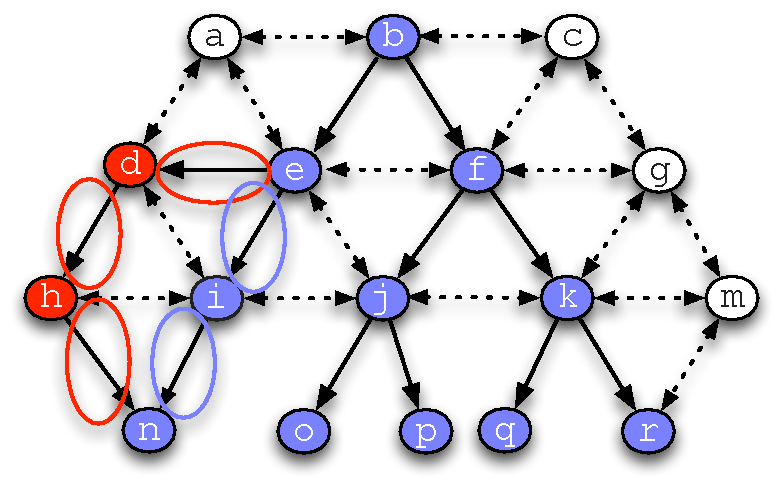
\includegraphics[scale=0.51]{figs/min-control-directed-example.pdf}
%\caption{Primary tree $T^l$ and backup tree, $\hat{T}^l$, where $l=(e,i)$. Edges unique to $T^l$ are circled in blue and unique $\hat{T}^l$ edges are circled in red. 
%$V^l \setminus \hat{V}^l = \{i\}$ and $\hat{V}^l \setminus V^l = \{d,h\}$. }
%\label{fig:min-control-example}
%\end{figure}


{\bf \pre \textsc{Algorithm.}}
\pre computes and installs backup tree flow table entries \emph{before} a primary tree link, $l$, fails.  After $l$ fails, \pre signals the backup tree root
to install a forwarding rule that activates the backup tree.  We use the term ``activate'' to indicated that packets are multicasted using the backup tree rather than the primary tree.

%as opposed to \post that requires signaling multiple nodes to install a backup tree, \pre yields faster recovery than \posts. 

\pre cannot, without modifications, pre-install basic flow table entries at all nodes because incorrect forwarding would result. Doing so at a node, $d$, common to the primary and backup tree,
where the backup and primary tree have different outgoing links, would either result in packets erroneously forwarded at $d$ using the backup tree before a link failure occurs or 
incorrectly forwarding packets using the primary tree after the link failure. 
We say that $d \in D^l$, where $D^l$ contains each node with one or more outgoing links in $T^l$ and one or more outgoing links in $\hat{T}^l \setminus T^l$.
Revisiting $\hat{T}_c$ from Figure \ref{fig:intuition-example} example, $g,m \in D^l$ and so installing a forwarding rule at these two switches before $(g,l)$ fails 
would be problematic for the reasons just described.
%Revisiting the Figure \ref{fig:intuition-example} example, installing a $\hat{T}_c$ forwarding rule at $g$ and $m$ before $(g,l)$ fails would be problematic for the reasons just described.


%Because $e$ has an outgoing link $(e,i) \in T^l$ and another outgoing link $(e,d)$ unique to $\hat{T}^l$,
%pre-installing $\hat{T}^l$'s flow table entry at $e$ would cause incorrect forwarding for either $T^l$ or $\hat{T}^l$.  
%We say that $e \in D^l$, where $D^l$ contains each node with one or more outgoing links in $T^l$ and one or more outgoing links in $\hat{T}^l \setminus T^l$.

%{\it [TODO: Missing description of how root node is signaled to write the {\tt bid}. ]}

To address this issue, \pre assigns a unique \emph{backup tree id}, denoted {\tt bid}, to each backup tree.  For each $d \in D^l$, the flow table entry matches and forwards packets
using the {\tt bid} value written in the {\tt dl\_src} field. When the backup tree $\hat{T}^l$ is activated, \pre writes the {\tt bid} in the
{\tt dl\_src} packet header field, indicating that these packets should be disseminated by $\hat{T}^l$ rather than $T^l$.
In more detail, \pre preinstalls and activates $\hat{T}^l$ using the following steps, where we assume $\hat{T}^l$ has {\tt bid=AA}:
\begin{enumerate}
	%\item Computes $D^l$.
	
	\item At each $d \in D^l$, \pre pre-installs a flow table entry matching packets using $\hat{T}^l$'s multicast address, {\tt dl\_src = AA}, and wildcards for all other match fields. 
	%\footnote{We assume $T^l$ has multicast address \mdsts.}
	
	\item Preinstalls a basic flow table entry at each $b \in B^l \setminus D^l$.

	\item When it is detected that $l$ fails, \pre installs a rule at the $\hat{T}^l$ root node that writes {\tt AA} in the {\tt dl\_src} header field of each $\hat{T}^l$ packet.
	%$e_r$ is given a higher priority than any other rule installed at $r$.
\end{enumerate}

For $\hat{T}_c$ in Figure \ref{fig:intuition-example}, \pre pre-installs a forwarding rule at $g$ and $m$ that matches packets using $\hat{T}_c$'s {\tt bid}, {\tt CC}, and $T_c$'s multicast 
address.  After $(g,l)$ fails, \pre signals $c$ to write {\tt CC} in the {\tt dl\_src} header field of each $\hat{T}_c$ packet.  As a result, packets at $g$ are correctly forwarded to
$m$ and, similarity, $m$ correctly forwards packets to $l$, $n$, and $t$.

{\bf Comparing \pre and \posts.}
Since \pre must signal only a single node, as opposed to multiple nodes with \posts, to install a backup tree, \pre is fast. However, \pres's speed comes at the cost of 
storing a potentially large number of flow table entries at the switches, especially since \mdr computes, for each primary tree, a backup tree for each primary tree link. \post, on the other hand,
only installs backup tree flow table entries after a link failure is detected.
These trade-offs are studied in Section \ref{sec:evaluation} using simulations.

%\post installs backup tree forwarding rules after a link failure is detected, while \pre installs backup tree flow table entries before a link failure occurs. With \pres, the backup 
%trees are only activated -- by writing an identifier in each packet header signaling packets to be routed using the backup tree -- after the link failure is detected.

%\pre requires that only the root node needs to be signaled to install a backup tree, at the cost of storing unused flow table entries (i.e., backup tree flow table entries installed before link 
%failures occur).  In contrast, because backup tree flow table entries are not preinstalled, \post introduces no storage overhead. However, multiple nodes must be signaled 
%to install a backup tree with \posts.
%and does not need tree ids to differentiate between primary tree and backup tree flow rules. % However, this comes at the cost of signaling overhead as each $B^l$ node must be signaled.


